\section{Performance Testing Environment} % (fold)
\label{sec:performance_testing_environment}
TODO: Machine specs, software versions, etc.

TODO: Benchmarkjs, uncertainties calculation.
% section performance_testing_environment (end)

\section{Application Performance Evaluation} % (fold)
\label{sec:application_performance_evaluation}
\subsection{Bullet Physics Performance} % (fold)
\label{sub:bullet_physics_performance}
The simplest way to measure how well the physics engine performs using Native Calls RPC is to analyse the frames per second for a range of scenes of varying complexity. We identify what is the biggest impact to the frames per second by measuring how long it takes to make a request and get a response for each frame rendered. We also measure how long it takes to perform the actual simulation step. Finally, we compare these measurements with the original implementation, which was implemented using Native Client Acceleration Modules and tweaked for performance using ArrayBuffers.

\subsubsection{Results and comparison} % (fold)
\label{ssub:results_bullet_physics_performance}
\begin{table}[h]
\begin{tabular}{lllll}
\multirow{2}{*}{Scene}               & \multicolumn{3}{l}{Time /ms}              & \multirow{2}{*}{Frames per second} \\
                                     & Frame Rendering & Round trip & Simulation &                                    \\ \hline
\multicolumn{1}{l|}{10 Jenga Blocks} & 16.90           & 16.67      & 0.08       & 60                                 \\
\multicolumn{1}{l|}{20 Jenga Blocks} & 16.95           & 16.54      & 1.17       & 55                                 \\
\multicolumn{1}{l|}{Random Shapes}   & 16.95           & 16.39      & 0.67       & 60                                 \\
\multicolumn{1}{l|}{250 Cubes}       & 16.95           & 16.39      & 1.67       & 60                                 \\
\multicolumn{1}{l|}{500 Cylinders}   & 24.39           & 21.74      & 4.93       & 54                                 \\
\multicolumn{1}{l|}{1000 Cubes}      & 37.04           & 37.04      & 10.97      & 32                                 \\
\multicolumn{1}{l|}{2000 Cubes}      & 66.67           & 66.67      & 26.94      & 18                                 \\
                                     &                 &            &            &                                    \\
                                     &                 &            &            &                                   
\end{tabular}
\caption{Bullet physics performance using Native Calls implementation}
\end{table}

Note, the numbers shown above show the amount of time and frame rate at the lowest point when the scene is rendering. Due to the nature of the simulation, the simulation time can vary depending on the scene. To illustrate this, Figure \ref{fig:graph-1k-cubes-nativecalls} shows a graph of milliseconds against time. The arrow points at the time when 1000 cubes were loaded into the scene. We can see the jump of the round trip time, where it seems to level off at around 37 milliseconds. But the physics simulation time goes up as the physics simulation becomes more complex. For example, at 15:41:30, the graph levels off at around 10 milliseconds. This gives us an indication as to what is most affecting the frame rate. In this case, it is mostly the framework time as opposed to the simulation time.

When we analyse a similar graph but this time for 2000 cubes, shown in Figure \ref{fig:graph-2k-cubes-nativecalls}, we can see a significant increase in the simulation time. This time, both the framework and the simulation time are bottle necks to the frame rate. However, when the 2000 cubes are no longer moving / interacting (they are now stationary on the floor), we can see in Figure \ref{fig:graph-2k-cubes-nativecalls-leveling} that obviously the main bottle neck is the RPC framework.

\begin{figure}
    \centering
    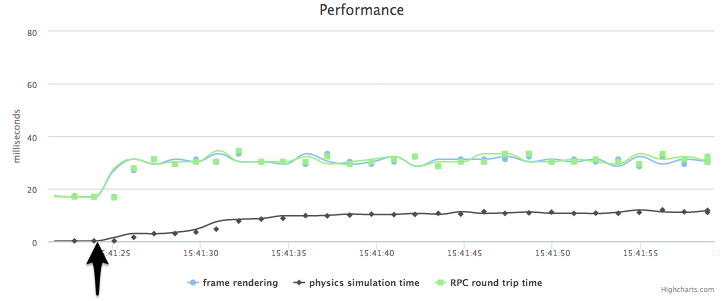
\includegraphics[width=1\textwidth]{graph-1k-cubes-nativecalls.png} 
    \caption{Graph showing contributing factors to the frame rate, when simulating 1000 cubes falling from the sky using Native Calls}
    \label{fig:graph-1k-cubes-nativecalls}
\end{figure}

\begin{figure}
    \centering
    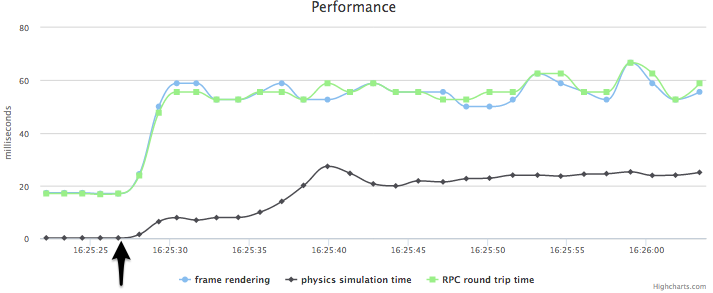
\includegraphics[width=1\textwidth]{graph-2k-cubes-nativecalls.png} 
    \caption{Graph showing contributing factors to the frame rate, when simulating 2000 cubes falling from the sky using Native Calls}
    \label{fig:graph-2k-cubes-nativecalls}
\end{figure}

\begin{figure}
    \centering
    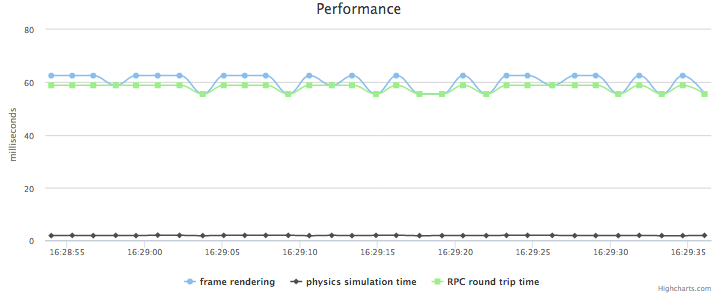
\includegraphics[width=1\textwidth]{graph-2k-cubes-nativecalls-leveling.png} 
    \caption{Graph showing contributing factors to the frame rate, when simulating 2000 cubes stationary on the floor using Native Calls}
    \label{fig:graph-2k-cubes-nativecalls-leveling}
\end{figure}


We now compare these results with the NaClAM implementation. For more information about how the NaClAM implementation works, you can read the related work section \ref{sec:naclam} on page \pageref{sec:naclam}. The table below shows the time taken for the NaClAM module to simulate the same scenes as before.

\begin{table}[h]
\begin{tabular}{lllll}
\multirow{2}{*}{Scene}               & \multicolumn{3}{l}{Time /ms}              & \multirow{2}{*}{Frames per second} \\
                                     & Frame Rendering & Round trip & Simulation &                                    \\ \hline
\multicolumn{1}{l|}{10 Jenga Blocks} & 16.90           & 16.90      & 0.11       & 60                                 \\
\multicolumn{1}{l|}{20 Jenga Blocks} & 16.95           & 16.95      & 0.12       & 60                                 \\
\multicolumn{1}{l|}{Random Shapes}   & 16.95           & 16.39      & 0.62       & 59                                 \\
\multicolumn{1}{l|}{250 Cubes}       & 16.95           & 16.39      & 1.62       & 60                                 \\
\multicolumn{1}{l|}{500 Cylinders}   & 17.54           & 21.74      & 5.45       & 59                                 \\
\multicolumn{1}{l|}{1000 Cubes}      & 17.54           & 37.04      & 11.76      & 57                                 \\
\multicolumn{1}{l|}{2000 Cubes}      & 29.41           & 31.78      & 25.75      & 40                                 \\
                                     &                 &            &            &                                    \\
                                     &                 &            &            &                                   
\end{tabular}
\caption{Bullet physics performance using NaClAM implementation}
\end{table}

Notice how the simulation time is more or less the same for both implementation. This makes sense, since both implementations have more or less the same C++ implementation.

We can also see that the main bottle neck to performance in this implementation is the simulation time, and not the RPC framework. This can be seen clearly from the graph in Figure \ref{fig:graph-2k-cubes-naclam}.

\begin{figure}
    \centering
    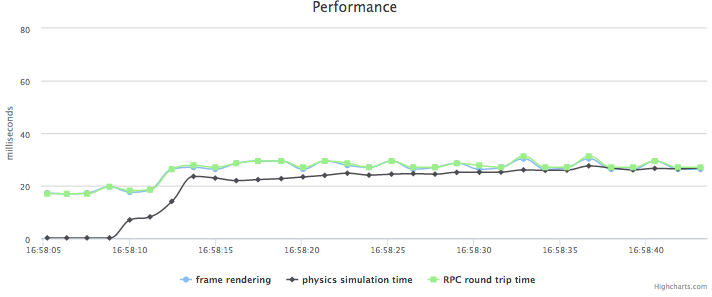
\includegraphics[width=1\textwidth]{graph-2k-cubes-naclam.png} 
    \caption{Graph showing contributing factors to the frame rate, when simulating 2000 cubes falling from the sky using NaClAM}
    \label{fig:graph-2k-cubes-naclam}
\end{figure}

% subsubsection results_bullet_physics_performance (end)

\subsubsection{Analysis} % (fold)
\label{ssub:bullet_physics_performanceanalysis}
From the graphs and tables, we can obviously see how the performance impact of our framework gets higher and higher with more and more objects being sent. We can see how, for large scenes such as 2000 cubes, the Native Calls implementation performs almost two times worse than the NaClAM implementation. However, for smaller scenes, the two implementations have very similar performance.

The most likely reason for this is because of the data marshalling on the C++ Native Calls RPC framework implementation. In our implementation, the data is processed in O(n) time in order to convert the received \lstinline{pp::VarArray} array of objects into a \lstinline{std::vector} of \lstinline{struct}s. In section \ref{sec:performance_evaluation} (page \pageref{sec:performance_evaluation}), we find that converting WebIDL dictionaries is also quite slow, compared to converting an array of numbers. When we compare this to the NaClAM implementation, we can see that the NaClAM version has almost O(1) time, since the data is only being read and is shared between the module and JavaScript. This is explained in section \ref{sec:naclam} on page \pageref{sec:naclam}.
% subsubsection bullet_physics_performanceanalysis (end)


\subsubsection{Implementation} % (fold)
\label{ssub:implementation_bullet_physics_performance}
The actual implementation of the RPC library for the physics simulation is discussed in the qualitative evaluation section. Here we discuss how we measure and plot the data that we saw in the tables and graphs above.

We measure three things - the frame rate, the simulation time, and the round trip time. To measure the frame rate, we simply add to a total of frames requested. A frame is requested by the browser automatically in order to achieve a frame rate of 60 frames per second. This is done using the \lstinline{window.requestAnimationFrame} API, which conveniently takes the computation time for rendering and processing the frame into account. This is why the frame rate drops when the round trip time and simulation time increases. We measure the total simulation time inside the C++ application by taking time stamps between and after the simulation step and calculating the difference. We send it back with the results every time we do the simulation. Finally, we calculate the round trip time by taking timestamps before and after the RPC call and taking a difference. We average all this data over a period of one second and send it to be plotted.

The graph is plotted in real time in the browser, but we make sure not to use the same \lstinline{window} object - as this will impact JavaScript performance and give us skewed results. Instead, we send the data to be plotted in a different window - which in Chrome corresponds to a different process. HighCharts was chosen to quickly and easily create the realtime graph with very little configuration. The demo and performance graphs are available on GitHub.

% subsubsection implementation_bullet_physics_performance (end)

% subsection bullet_physics_performance (end)

\subsection{Oniguruma Regular Expressions Performance} % (fold)
\label{sub:oniguruma_regular_expressions_performance}
To get an insight of the performance of the oniguruma library for Native Client using Native Calls, we shall count the number of regular expression matches. We compare this to running the engine in Node JS server natively, and then using WebSockets to get functionality in the browser.

\subsubsection{Results and comparison} % (fold)
\label{ssub:onig_results_and_comparison}
TODO
% subsubsection onig_results_and_comparison (end)

\subsubsection{Analysis} % (fold)
\label{ssub:onig_analysis}
TODO
% subsubsection onig_analysis (end)

\subsubsection{Implementation} % (fold)
\label{ssub:onig_implementation}
Again, the actual implementation of the library is discussed later on in the evaluation. In this section, we discuss how we measure the number of matches.

TODO.
% subsubsection onig_implementation (end)

% subsection oniguruma_regular_expressions_performance (end)
% section application_performance_evaluation (end)

\section{Framework Performance Evaluation} % (fold)
\label{sec:performance_evaluation}
We used the IDL file shown in Listing \ref{code_webidl_benchmarks} to test transfer and processing performance of individual operations:

\lstset{language=C,caption={WebIDL file used for benchmarking},label=code_webidl_benchmarks}
\begin{code}
dictionary dict {
  DOMString str;
  double d;
  boolean b;
};

dictionary nestedDict {
  DOMString topStr;
  double topD;
  boolean topB;
  dict nested;
};

interface Benchmark{
  long bench_long(long v);
  double bench_double(double v);
  DOMString bench_DOMString(DOMString v);
  dict bench_dict(dict v);
  nestedDict bench_nestedDict(nestedDict v);

  sequence<long> bench_seq_long(sequence<long> v);
  sequence<double> bench_seq_double(sequence<double> v);
  sequence<DOMString> bench_seq_DOMString(sequence<DOMString> v);
  sequence<dict> bench_seq_dict(sequence<dict> v);
  sequence<nestedDict> bench_seq_nestedDict(sequence<nestedDict> v);
};
\end{code}

We will use the generated RPC library to test the framework's performance. We will do this by making RPC calls and measuring how long it takes.

\subsection{Round trip performance}\label{round-trip-performance}

We measure the number of round trips performed in one second (round trips per second, RT/s).

One round trip corresponds to a full remote procedure call, starting from JavaScript, reaching the target function, returning from the function, and going back to the JavaScript. This is illustrated in Figure \ref{fig:rpc_roundtrip}.


\begin{figure}
    \centering
    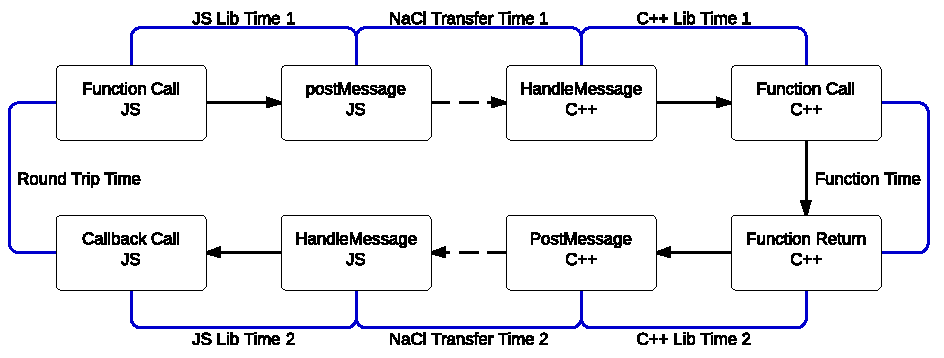
\includegraphics[width=1\textwidth]{RoundTrip.pdf} 
    \caption{A depiction of the round trip time from JavaScript to C++}
    \label{fig:rpc_roundtrip}
\end{figure}


\begin{table}[h]
\begin{tabular}{l|lll}
\textbf{Type}       & \textbf{Mean RT/s} & \textbf{Uncertainty} & \textbf{Number of runs} \\ \hline
\textbf{long}       & 418                & $\pm$1.79\%              & 56                      \\
\textbf{double}     & 423                & $\pm$2.08\%              & 48                      \\
\textbf{DOMString}  & 420                & $\pm$1.25\%              & 43                      \\
\textbf{dict}       & 415                & $\pm$2.39\%              & 44                      \\
\textbf{nestedDict} & 385                & $\pm$1.29\%              & 47                     
\end{tabular}
\caption{Round trip performance of sending a single parameter}
\label{table:roundtrip_single_param}
\end{table}


\begin{table}[h]
\begin{tabular}{l|lllll}
\multirow{2}{*}{\textbf{Array Length}} & \multicolumn{5}{l}{\textbf{Round trips per second}}                                        \\
                                       & \textbf{long} & \textbf{double} & \textbf{DOMString} & \textbf{dict} & \textbf{nestedDict} \\ \hline
\textbf{10}                            & 403 $\pm$2.20\%   & 403 $\pm$2.19\%     & 378 $\pm$1.48\%        & 317 $\pm$1.76\%   & 244 $\pm$1.81\%         \\
\textbf{45}                            & 379 $\pm$1.99\%   & 384 $\pm$2.01\%     & 309 $\pm$1.22\%        & 182 $\pm$3.03\%   & 112 $\pm$1.15\%         \\
\textbf{100}                           & 354 $\pm$2.01\%   & 347 $\pm$1.62\%     & 234 $\pm$2.59\%        & 110 $\pm$1.36\%   & 60.07 $\pm$1.24\%       \\
\textbf{450}                           & 237 $\pm$1.18\%   & 235 $\pm$2.07\%     & 102 $\pm$1.48\%        & 32.82 $\pm$1.10\% & 15.83 $\pm$0.96\%       \\
\textbf{1000}                          & 163 $\pm$1.54\%   & 160 $\pm$1.04\%     & 55.41 $\pm$1.89\%      & 15.39 $\pm$1.06\% & 7.43 $\pm$1.29\%        \\
\textbf{4500}                          & 49.39 $\pm$1.67\% & 48.93 $\pm$1.41\%   & 14.60 $\pm$0.75\%      & 3.62 $\pm$1.26\%  & 1.68 $\pm$1.05\%        \\
\textbf{10000}                         & 24.68 $\pm$0.90\% & 24.50 $\pm$1.00\%   & 6.62 $\pm$1.85\%       & 1.62 $\pm$1.68\%  & 0.75 $\pm$1.81\%        \\
\textbf{45000}                         & 5.99 $\pm$1.37\%  & 5.98 $\pm$0.92\%    & 1.28 $\pm$2.92\%       & 0.33 $\pm$2.48\%  & 0.15 $\pm$2.46\%       
\end{tabular}
\caption{Round trip performance for arrays of different lengths and types}
\label{table:roundtrip_array}
\end{table}

Tables \ref{table:roundtrip_array} and \ref{table:roundtrip_single_param} show the number of round trips performed in a second for RPC calls with a single parameter and different array lengths. To compare these times, Figure \ref{fig:arraylength-time-plot} shows a column chart visualisation of the data.

\begin{figure}
    \centering
    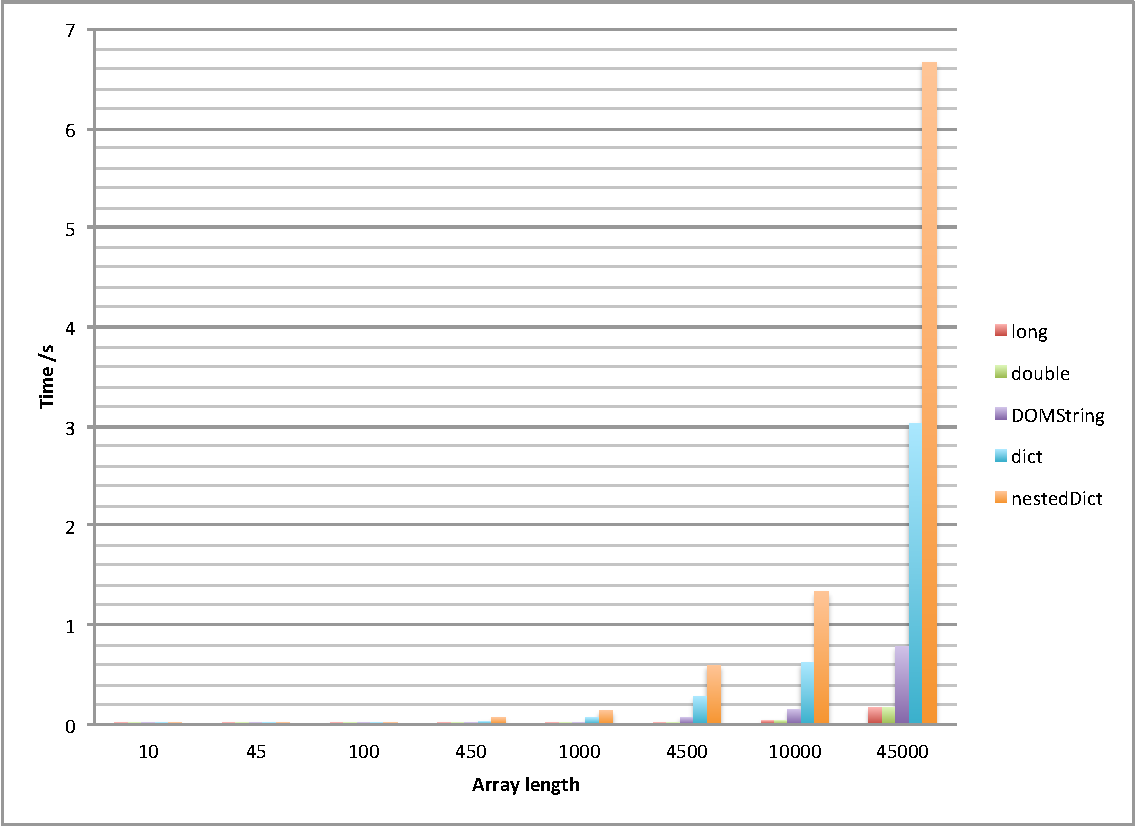
\includegraphics[width=1\textwidth]{arraylength-time-plot.pdf} 
    \caption{The round trip time for arrays of different lengths and types}
    \label{fig:arraylength-time-plot}
\end{figure}


\begin{figure}
    \centering
    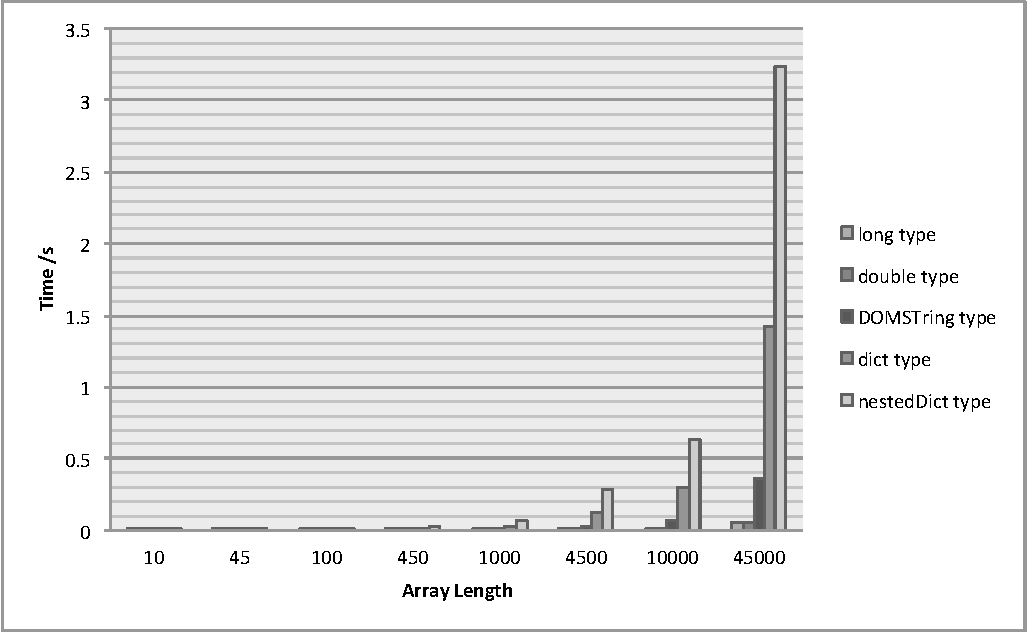
\includegraphics[width=1\textwidth]{arraylength-time-cpp-plot.pdf} 
    \caption{The C++ library time for arrays of different lengths and types}
    \label{fig:arraylength-time-cpp-plot}
\end{figure}



\subsection{C++ Library Time}\label{c-library-time}

We measure the number of microseconds taken to handle a RPC call. This is
the time it takes to detect it is an RPC call, extract parameters,
convert them, find the method, call it, pack the result, and post the
message back to JS.

The results are measured and averaged for the same runs that were
performed above. Tables \ref{table:cpp_lib_time_single_param} and \ref{table:cpp_lib_time_arrays} show the results, and Figure \ref{fig:arraylength-time-cpp-plot} shows a visualisation of the data.


\begin{table}[h]
\begin{tabular}{l|ll}
\textbf{Type}       & \textbf{Mean lib time/$\mu$s} & \textbf{Uncertainty (1 sd)} \\ \hline
\textbf{long}       & 105.50                    & 17.88                       \\
\textbf{double}     & 104.12                    & 17.34                       \\
\textbf{DOMString}  & 103.98                    & 17.55                       \\
\textbf{dict}       & 136.15                    & 23.35                       \\
\textbf{nestedDict} & 179.71                    & 28.32                      
\end{tabular}
\caption{Mean C++ library time for sending and receiving single parameters of different types}
\label{table:cpp_lib_time_single_param}
\end{table}


\begin{table}[h]
\begin{tabular}{l|lllll}
\multirow{2}{*}{\textbf{Array Length}} & \multicolumn{5}{l}{\textbf{Time / $\mu$s}}                                                                             \\
                                       & \textbf{long} & \textbf{double} & \textbf{DOMSTring} & \textbf{dict} & \textbf{nestedDict} \\ \hline
\textbf{10}                            & 125.40             & 125.91               & 197.42                  & 453.41             & 861.02                   \\
\textbf{45}                            & 168.64             & 163.34               & 484.03                  & 1512.79            & 3272.52                  \\
\textbf{100}                           & 242.70             & 245.74               & 906.05                  & 3445.17            & 7009.90                  \\
\textbf{450}                           & 705.10             & 703.79               & 3734.62                 & 13628.62           & 28198.18                 \\
\textbf{1000}                          & 1275.59            & 1354.86              & 7606.78                 & 29582.43           & 63493.50                 \\
\textbf{4500}                          & 5547.10            & 5564.47              & 30485.21                & 132121.82          & 292827.69                \\
\textbf{10000}                         & 11282.88           & 11376.26             & 68443.89                & 301437.50          & 632956.25                \\
\textbf{45000}                         & 50532.42           & 50843.33             & 359133.64               & 1418791.67         & 3242286.00               \\
\textbf{100000}                        & 104087.22          & 114020.00            & 799742.86               & 3319250.00         & 7347985.00              
\end{tabular}
\caption{Mean C++ library time for sending and receiving arrays of different lengths and types}
\label{table:cpp_lib_time_arrays}
\end{table}

\subsection{JS Library performance}\label{js-library-performance}

The JS library performance \textbf{without} validation has also been
measured, however its performance impact is negligible. The slowest
benchmark was found to take approx 3 microseconds (269,253 ops/sec
$\pm$  1.90\%).

\subsection{Analysis}\label{analysis}

From the data, we can see that for small types, the most contributing
factor to performance is the browser (e.g.~event system, etc.) and PPAPI
libraries (how PPAPI implements postMessage). For example, sending a
single long type takes 2392.34 microseconds (.002 seconds), but our
library only spends 105.5 microseconds processing the call (less than
5\% of the time).

For large and complicated data, the impact of using the library becomes
higher and higher. For example, sending 45000 nested objects (which are
actually quite simple) has a total round-trip time of 6.67s, and a whole
3.24 seconds of this is spent in our library (i.e.~half the time).

The most likely reason for this is that the C++ library takes O(n) time to process the data in order to marshal it, by converting it from a \lstinline{pp::VarArray} into a \lstinline{std::vector}.

TODO: Reasons why DOMString and dictionaries take longer than other types?

% section performance_evaluation (end)